\subsection{The 3morduc platform}
\label{sec:3morduc}

\begin{figure} [h]
  \begin{center}
    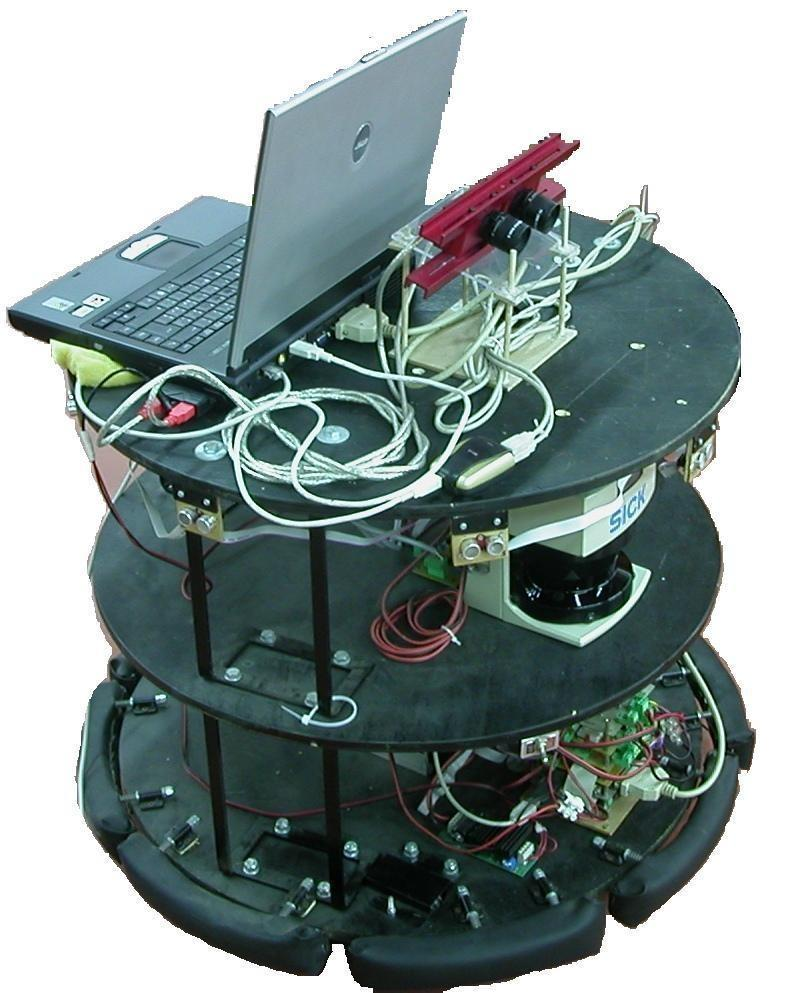
\includegraphics[width=150pt]{img/3morduc.jpg}
    \caption{The 3morduc robotic platform}
    \label{fig:morduc}
  \end{center}
\end{figure}

The telerobot used to develop teleoperation research is
called \textit{3MO.R.D.U.C.}, acronym for `3rd version of
the Mobile Robot DIEES University of Catania'.
3morduc is a mobile-robot, able to move forward, backward
and turn its direction, as directed by the remote operator.
It has been successfully used in several test and experimental
work regarding teleoperation and telepresence.
\\
The robot, actually located at the University of
Catania, is a differential-driven mobile robot, showed
in figure \ref{fig:morduc}.
\\
As every mobile robot, it is equipped with some internal
and external sensors, through which is possible retrieve
information about, respectively, the status of the robot
(e.g. its position) or the data about the environment (e.g.
distance from obstacles).

\subsubsection{Sensors and actuators}
\label{sec:3morduc:sensors_actuators}


The movement is performed by means of two 40W DC engines, model
\textit{Maxon F2260}, connected with the motor shaft by a gear
box (transmission rate 1/19). On the other side the motor shaft
is linked with two rubber wheels, while a third castor wheel can
freely turn to realize the differential-driven model.
\\
The robot is compound by three shelves, each one connected to
the next. On the lower level two lead batteries are situated,
able to erogate 12 Volts at 18 Amperes. The electrical autonomy is
granted for 30-40 minutes.
\begin{figure}[h]
  \begin{center}
    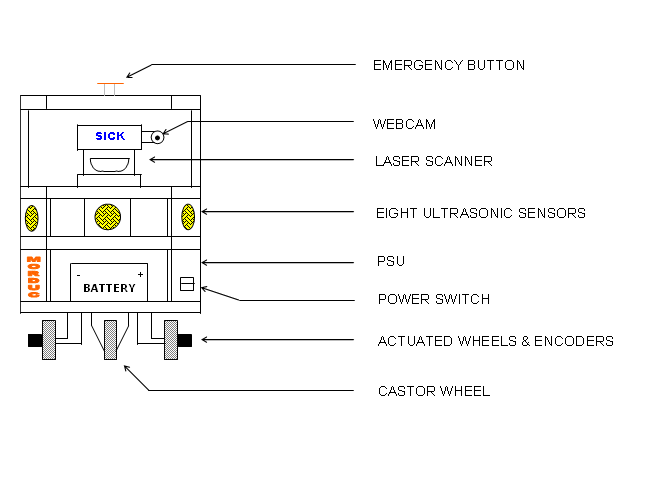
\includegraphics[width=300pt]{img/Morduc_scheme.png}
    \caption{3morduc's schematic figure}
    \label{fig:morduc_scheme}
  \end{center}
\end{figure}
\\
Besides, on the same lower level is located an electronic board
controlling different modules, each one predisposed to manage a
specific task as movements, sensors and communication.
\\
Type and number of sensors available on 3morduc are:

\begin{itemize}
\item \texttt{belt of bumpers} \\
  A belt of bumpers (in total 16 switches) is dislocated around
  the entire perimeter on the robot base, just over the wheels level. \\
  See chapter \textit{Bumper} (\ref{sec:mobile:bumper}) for more details
  about this type of sensor.

\item \texttt{incremental encoders} \\
  The two robot motor axes are equipped with incremental encoders, with
  resolution of 500 pulses per turn. These sensors are useful to calculate
  heading and position of the robot by using the kinematic model. \\  
  See chapter \textit{Encoder} (\ref{sec:mobile:encoder}) for more details
  about this type of sensor.
 
\item \texttt{belt of sonars} \\
  On the second level are located eight sonar sensors, which measure the
  distance from an obstacle using the flight time of an ultrasonic signal
  produced by means of a vibrating piezoelectric sensor. \\
  See chapter \textit{Sonar} (\ref{sec:mobile:sonar}) for more details
  about this type of sensor.

\item \texttt{scanner laser} \\
  In order to detect obstacles on the workspace, the \textit{Laser Measurement
  Sensor} (LMS) operates by measuring the flight time of a pulsed laser
  light beam that is reflected by obstacle, to provide a 2D scanning data. \\
  It is possible to configure different angular resolution (0.25\textdegree,
  0.5\textdegree or 1\textdegree pace) with different angular scan (100\textdegree
  or 180\textdegree).
  \begin{figure}[h]
    \begin{center}
      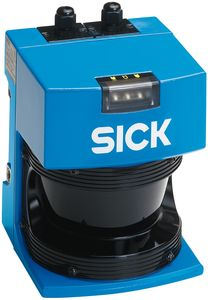
\includegraphics[width=60pt]{img/laser_sick_lms_200.jpg}
      \caption{LMS Sick mounted on 3morduc}
      \label{fig:laser_sick_lms_200}
    \end{center}
  \end{figure}
  \\
  See chapter \textit{Laser} (\ref{sec:mobile:laser}) for more details
  about this type of sensor. The reference manual about \textit{LMS
  Sick 200} can be found at \cite{3morduc:laser_sick_200}.

\item \texttt{stereo cameras} \\
  On the robot there are also two stereoscopic cameras, each one with a
  resolution of 1.3 megapixel and fixed focus lens of 4.0 mm. \\
  The CCD sensors of these cameras have a good noise immunity and
  sensibility; moreover, it is possible to adjust all the image parameter, e.g.
  exposure gain, frame rate, resolution. \\
  The cameras are mounted on a rigid support; it permits to simply adjust
  the camera distance in a range 5-20 cm. \\
  Both the cameras can be connected to PC by IEEE 1394 interface, with a
  frequency of synchronization of 8 KHz. \\
  \begin{figure}[h]
    \begin{center}
      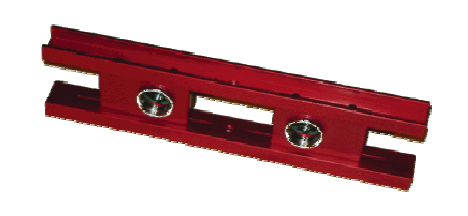
\includegraphics[width=200pt]{img/camera_videre.png}
      \caption{STH-MDCS2-VAR-C mounted on 3morduc}
      \label{fig:camera_videre}
    \end{center}
  \end{figure}
  \\
  See chapter \textit{Image sensors} (\ref{sec:mobile:image}) for more details
  about this type of sensor. The reference manual about the \textit{STH-MDCS2-VAR-C}
  can be found at \cite{3morduc:camera_sth_mdcs2}.

  

\end{itemize}

More images, video and information about 3morduc can
be found at \cite{morduc:features}.


\subsubsection{Internet communication}
\label{sec:3morduc:communication}

The network system implemented on the 3morduc is a typical
client-server architecture: in order to control the robot through
Internet, 3morduc implements an HTTP server.
\\
Through different type of prearranged HTTP requests, a generic
HTTP client sends command to the server and retrieve information
about 3morduc's status. In this way, client needs only to open a TCP/IP
socket on the HTTP standard port (number 80) to control the robot from
remote.
\begin{figure}[h]
  \begin{center}
    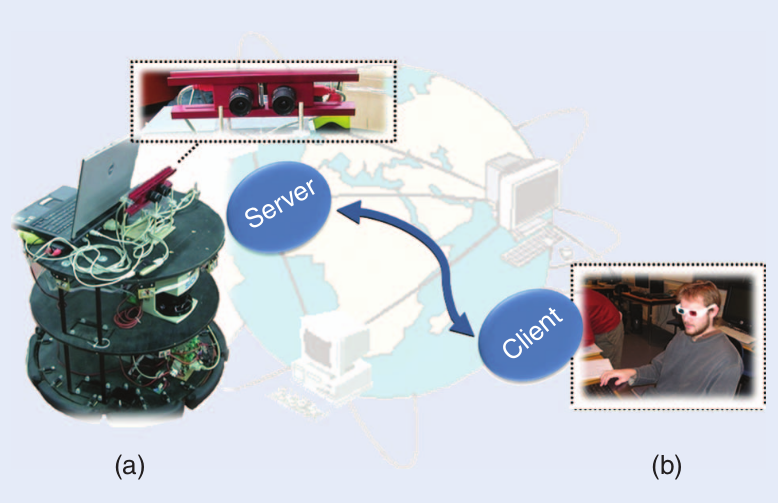
\includegraphics[width=300pt]{img/3morduc_client_server.png}
    \caption{A representation of the local-remote system
      interaction. (a) Mobile robot in Robotics Lab, University of
      Catania, Italy, equipped with a stereo camera and sitting on
      the platform, responsible for capturing stereo images or mono
      images. (b) User located in remote place, using a generic HTTP
      client to send command to the robot and receive its images
      and status data.
    }
    \label{fig:3morduc_client_server}
    \end{center}
\end{figure}
\\
The Server was developed in Borland \textit{Delphi 7}, an object oriented
language
derived by Pascal. Several classes are wrapper of the windows A.P.I., making
really simple to develop efficient code in fast way. The choice of this
programming language come from the necessity to include it as part of the
control system designed in Catania for the 3morduc robot.
\\
A first client was developed using \textit{MFC} (\textit{Microsoft Foundation
Classes}) in Visual C++ (with supporting framework \textit{Visual Studio 2005}).
It uses \textit{OpenGL} libraries to create 3D synthetic images and to handle
the different kinds of used VR instruments provided by the client platform.
For a specific study view \cite{morduc:neri}.
\\
Different clients has been developed after the one described above, aiming to
improve user's skill to move the robot in the remote environment
(some will be briefly described in \ref{sec:improvements_telepresence}). There are
clients tightly bound to Windows platform, and others
built on free libraries and multi-platform code (like C++), which makes clients
platform independent. The communication protocol chosen allows to
access the server through a standard interface: every programming language
allows to send and retrieve HTTP requests without any effort.
\\
We will survey now, more in details, messages exchange between client and server.
After creating a socket and opening the communication channel, client is able
to send request to 3morduc and receive correlated responses.
\\
Client request is built with only an HTTP header, without the body. The related
fields are listed in table \ref{table:header_request}.

\begin{table}[h]
  \centering  
  \begin{tabular}{| c | c |}

    \hline
    \texttt{\bf Header line} &
    \texttt{\bf Description} \\ %[0.5ex] 

    \hline
    \parbox[t]{6.5cm}{\raggedright \small GET http://$<$URL$>$ HTTP/1.1 $<$CLRF$>$} &
    \parbox[t]{6cm}{\raggedright \small
      Retrieve (execute) the document (action) identified by $<$URL$>$,
      using HTTP protocol version 1.1.} \\  [1ex]

    \hline
    \parbox[t]{6.5cm}{\raggedright \small Host: $<$HOST$>$ $<$CLRF$>$} &
    \parbox[t]{6cm}{\raggedright \small
      $<$HOST$>$ is the IP serve address to which route the request.} \\ [1ex]
    
    \hline
    \parbox[t]{6.5cm}{\raggedright \small User-agent:  $<$CLIENT$>$ $<$CLRF$>$} &
    \parbox[t]{6cm}{\raggedright \small
      $<$CLIENT$>$ is a string identifying the client. It is used for log
      purpose only.} \\  [1ex]

    \hline
    \parbox[t]{6.5cm}{\raggedright \small $<$CLRF$>$} &
    \parbox[t]{6cm}{\raggedright \small
      A black line to indicate HTTP header end.} \\ [1ex]

    \hline

  \end{tabular}
  \caption{HTTP header request structure.}
  \label{table:header_request}
\end{table}

Camera images are provided together as a unique 1280x480 pixels image, 
(by joining two images of 640x480, left and right).
\\
A laser map of the environment is a jpeg or bmp 200x200 image. The map-building
algorithm is based on the laser scanner sensor and produces a black/white image
map, where each pixel represents a square area 10cm x 10cm. A black pixel corresponds
to an obstacle, otherwise the space is free. The map-building algorithm used is a
classical `occupancy grid', based on the laser row data.
\\
Changing the requested URL (which is always directed to the same host,
i.e. the 3morduc server), client can submit three different type of request.
Every requested resorce matches a specific command, so a complete URL used
by the client will appear as:

\begin{center}
  \textit{http://MoruducIPAddress/URLResourceName}
\end{center}

The first requests' group allows client to fetch laser map or camera image and
immediately after command the robot. 3morduc can be moved
forward or backward with a fixed pace, while its direction can be turned
with a fixed angle (towards left or right, from camera point
of view). All these commands have the following structure:

\begin{center}
  \texttt{$<$image\_type$>$.$<$command$>$.$<$body\_format$>$}
\end{center}

where \\ \\
\textit{$<$image\_type$>$} can assume one of the value described in table
\ref{table:image_type};\\
\textit{$<$command$>$} can assume one of the value described in table
\ref{table:command_type};\\
\textit{$<$body\_format$>$} can assume one of the value described in table
\ref{table:body_format}. \\

\begin{table}[!h]
  \centering  
  \begin{tabular}{| c | c |}

    \hline
    \texttt{\bf Image type} &
    \texttt{\bf Description} \\ %[0.5ex] 

    \hline
    \parbox[t]{6.5cm}{\raggedright \small stereo } &
    \parbox[t]{6cm}{\raggedright \small
      Retrieve image from camera.} \\  [1ex]

    \hline
    \parbox[t]{6.5cm}{\raggedright \small laser } &
    \parbox[t]{6cm}{\raggedright \small
      Retrieve laser map image.} \\  [1ex]

    \hline
    \parbox[t]{6.5cm}{\raggedright \small  laserimg } &
    \parbox[t]{6cm}{\raggedright \small
      Retrieve image from camera and laser map in one frame.} \\  [1ex]

    \hline
    \parbox[t]{6.5cm}{\raggedright \small datilaserandImg } &
    \parbox[t]{6cm}{\raggedright \small
      Retrieve image from camera and data from laser in HTTP header response.} \\  [1ex]

    \hline

  \end{tabular}
  \caption{Image type field in URL.}
  \label{table:image_type}
\end{table}

\begin{table}[!h]
  \centering  
  \begin{tabular}{| c | c |}

    \hline
    \texttt{\bf Command type} &
    \texttt{\bf Description} \\ %[0.5ex] 

    \hline
    \parbox[t]{6.5cm}{\raggedright \small fow } &
    \parbox[t]{6cm}{\raggedright \small
      Move robot forward.} \\  [1ex]

    \hline
    \parbox[t]{6.5cm}{\raggedright \small bak } &
    \parbox[t]{6cm}{\raggedright \small
      Move robot backward.} \\  [1ex]

    \hline
    \parbox[t]{6.5cm}{\raggedright \small lft } &
    \parbox[t]{6cm}{\raggedright \small
      Turn robot direction to the left.} \\  [1ex]

    \hline
    \parbox[t]{6.5cm}{\raggedright \small rgh } &
    \parbox[t]{6cm}{\raggedright \small
      Turn robot direction to the right.} \\  [1ex]

    \hline

  \end{tabular}
  \caption{Command type field in URL.}
  \label{table:command_type}
\end{table}

\begin{table}[!h]
  \centering  
  \begin{tabular}{| c | c |}

    \hline
    \texttt{\bf Body format} &
    \texttt{\bf Description} \\ %[0.5ex] 

    \hline
    \parbox[t]{6.5cm}{\raggedright \small jpg } &
    \parbox[t]{6cm}{\raggedright \small
      To obtain jpeg image.} \\  [1ex]

    \hline
    \parbox[t]{6.5cm}{\raggedright \small bmp } &
    \parbox[t]{6cm}{\raggedright \small
      To obtain bmp image.} \\  [1ex]
    \hline

  \end{tabular}
  \caption{Body format field in URL.}
  \label{table:body_format}
\end{table}

Be careful that with the commands above user do not receiver last robot's image or
status data, because the provided information is relative to the moment
before robot executes the issued command.
\\
The second requests' group allows client to fetch laser map or camera image,
without submitting any command to the robot. In these case commands have
the following structure:

\begin{center}
  \texttt{$<$image\_type$>$.$<$body\_format$>$}
\end{center}

where \\ \\
\textit{$<$image\_type$>$} can assume one of the value described in table
\ref{table:image_type};\\
\textit{$<$body\_format$>$} can assume one of the value described in table
\ref{table:body_format}. \\
\\
Last command's group define an URL structure to issue commands to the robot
without requesting any image or data.

\begin{center}
  \texttt{$<$command$>$.$<$how$>$}
\end{center}

In this case all the possible valid URLs are:

\begin{itemize}
  \item \textit{step.fow} \\
    Move robot forward;
  \item \textit{step.bak} \\
    Move robot backward;
  \item \textit{turn.rgh} \\
    Turn robot to the right;
  \item \textit{turn.lft} \\
    Turn robot to the left;
\end{itemize}

On server side, 3morduc sends an acknowledge message as
request replay. Since this is an HTTP message, it contains an HTTP header and
an HTTP body. The former has always the structure summarized in table 
\ref{table:header_response}, with some exception.
\\
The `Data' field is included in HTTP header only if a `datilaserandImg'
value has been submitted as image type in the URL request. Moreover, if client
issue only a command without requesting any robot's image or data (the type
of commands belonging to the third group), the response HTTP body will carry
no information, so fields `Content-Length' and `Content-Type' will be missing.

\begin{table}[!h]
  \centering  
  \begin{tabular}{| c | c |}

    \hline
    \texttt{\bf Header line} &
    \texttt{\bf Description} \\ %[0.5ex] 

    \hline
    \parbox[t]{6.5cm}{\raggedright \small HTTP/1.1 200 OK $<$CLRF$>$} &
    \parbox[t]{6cm}{\raggedright \small
      HTTP implemented version is 1.1, the result code related to the request
      is 200 (that means everything went fine).} \\  [1ex]

    \hline
    \parbox[t]{6.5cm}{\raggedright \small Server:Morduc/t/x/y/theta/collision/
      mindist $<$CLRF$>$} &
    \parbox[t]{6cm}{\raggedright \small
      Returned values are:
      \break name of the server;
      \break \textit{t} time in millisecond;
      \break \textit{x} and \textit{y} abscissa and ordinate for robot position, in meters;
      \break \textit{theta} rotation angle, in degrees;
      \break \textit{collision} number of collisions;
      \break \textit{mindist} distance from nearest obstacle, in meter.} \\  [1ex]

    \hline
    \parbox[t]{6.5cm}{\raggedright \small Data: Laser/$<$laser\_data1$>$/
      $<$laser\_data2$>$/.../$<$laser\_data181$>$/ $<$CLRF$>$} &
    \parbox[t]{6cm}{\raggedright \small
      Distance measured with laser scanner, in meters. 
      Every scan sweeps 180\textdegree.} \\ [1ex]
    
    \hline
    \parbox[t]{6.5cm}{\raggedright \small Content-Type: image/jpeg $<$CLRF$>$} &
    \parbox[t]{6cm}{\raggedright \small
      HTTP body contains a jpeg image. This can be a 200x200 image if a laser map of
      the environment was requested, or a 1240x480 image (composed by two 640x480
      images, from right and left camera) if camera image was requested.} \\  [1ex]

    \hline
    \parbox[t]{6.5cm}{\raggedright \small Content-Length: $<$bytesnumber$>$ $<$CLRF$>$} &
    \parbox[t]{6cm}{\raggedright \small
      Image dimension, in byte.} \\  [1ex]

    \hline
    \parbox[t]{6.5cm}{\raggedright \small $<$CLRF$>$} &
    \parbox[t]{6cm}{\raggedright \small
      A black line to indicate HTTP header end.} \\ [1ex]

    \hline


  \end{tabular}
  \caption{HTTP header response structure.}
  \label{table:header_response}
\end{table}
